% Captions for the lake figures.
% Files in docs/1M/figures/:  lake_a.pdf, lake_b.pdf, lake_ab.pdf
% Regenerate with:  python -m ModelLakeFishing.viz.lake_ab
%
% Built from A0, split seed 0: export A0GD_full_s0_e25, graph acddeb93d926ef…,
% and the measured evaluation in a0_hnsw_s0.npz.  Every number below is printed
% by the command above -- it reports each figure's own frame count and the
% case's ranks -- so reconcile these lines against that output after a rebuild
% rather than trusting them.  As of this build: 3,016,439 model rows, 64,086
% outside the frame, 41,056 families with 17 named, the 1,000-candidate HNSW
% pool, the gold 445th on cosine alone and returned first.
%
% Six of the ten returned are general LLMs that the map places in the LLM
% region, far from the query.  That is the measured answer, not a framing
% artifact: the map is laid out by representation, so a disc's distance from
% the query is not its retrieval distance.
%
% Panel A takes the lake's own aspect (0.97 under A0) and panel B its cast's.
% Do not force either into a box of your own choosing: that is what used to
% leave the lake small and structureless in the middle of white paper.


% ------------------------------------------------------------------ A alone --
\begin{figure}[t]
  \centering
  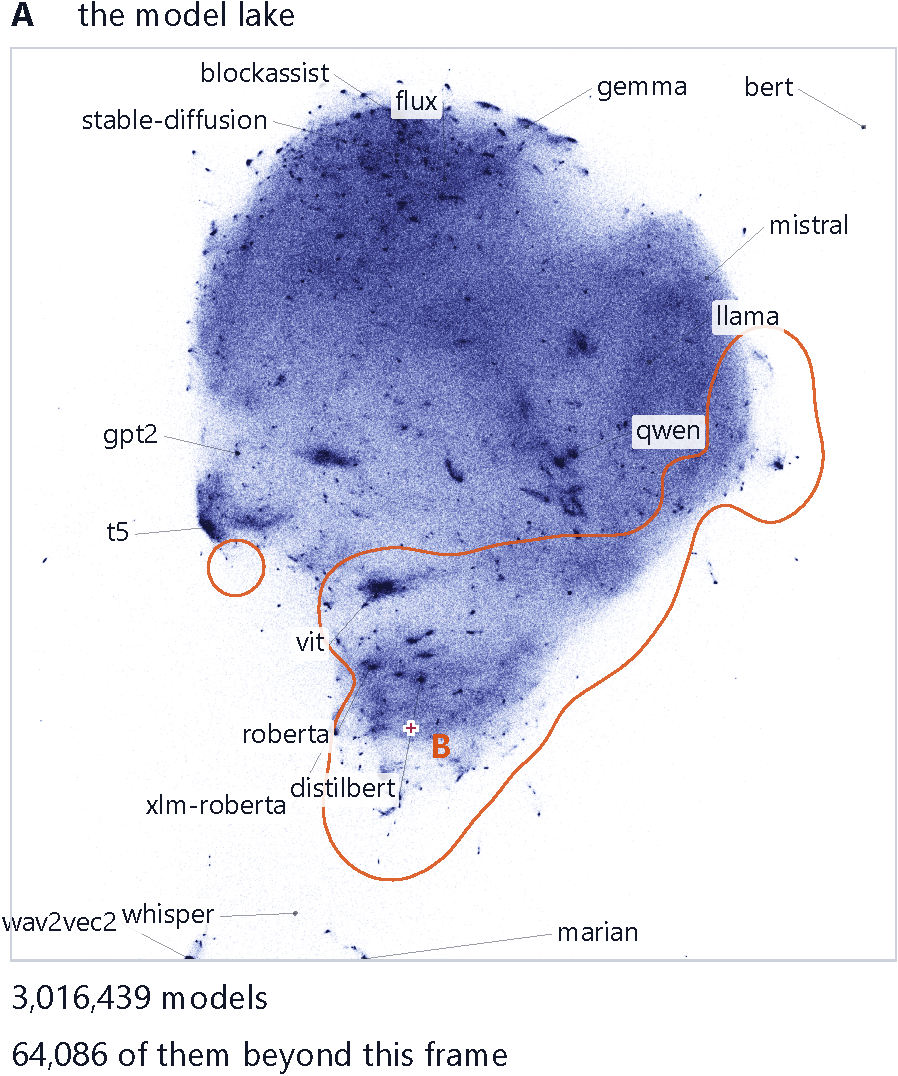
\includegraphics[width=\columnwidth]{figures/lake_a.pdf}
  \caption{%
    \textbf{The model lake.} All $3{,}016{,}439$ model representations laid
    out once, as log density over a UMAP projection of the shared
    $128$-dimensional retrieval space; $64{,}086$ rows fall outside the frame.
    Neighbourhoods are meaningful, absolute distances are not. Labels mark the
    densest region of $17$ of the $41{,}056$ model families. The crimson
    marker is one held-out query, \texttt{squad}\,/\,\emph{question-answering},
    and the amber outline encloses the region occupied by the $1{,}000$
    candidates HNSW retrieves for it: a bounded cast, but not a small
    neighbourhood.%
  }
  \label{fig:lake-a}
\end{figure}


% ------------------------------------------------------------------ B alone --
\begin{figure}[t]
  \centering
  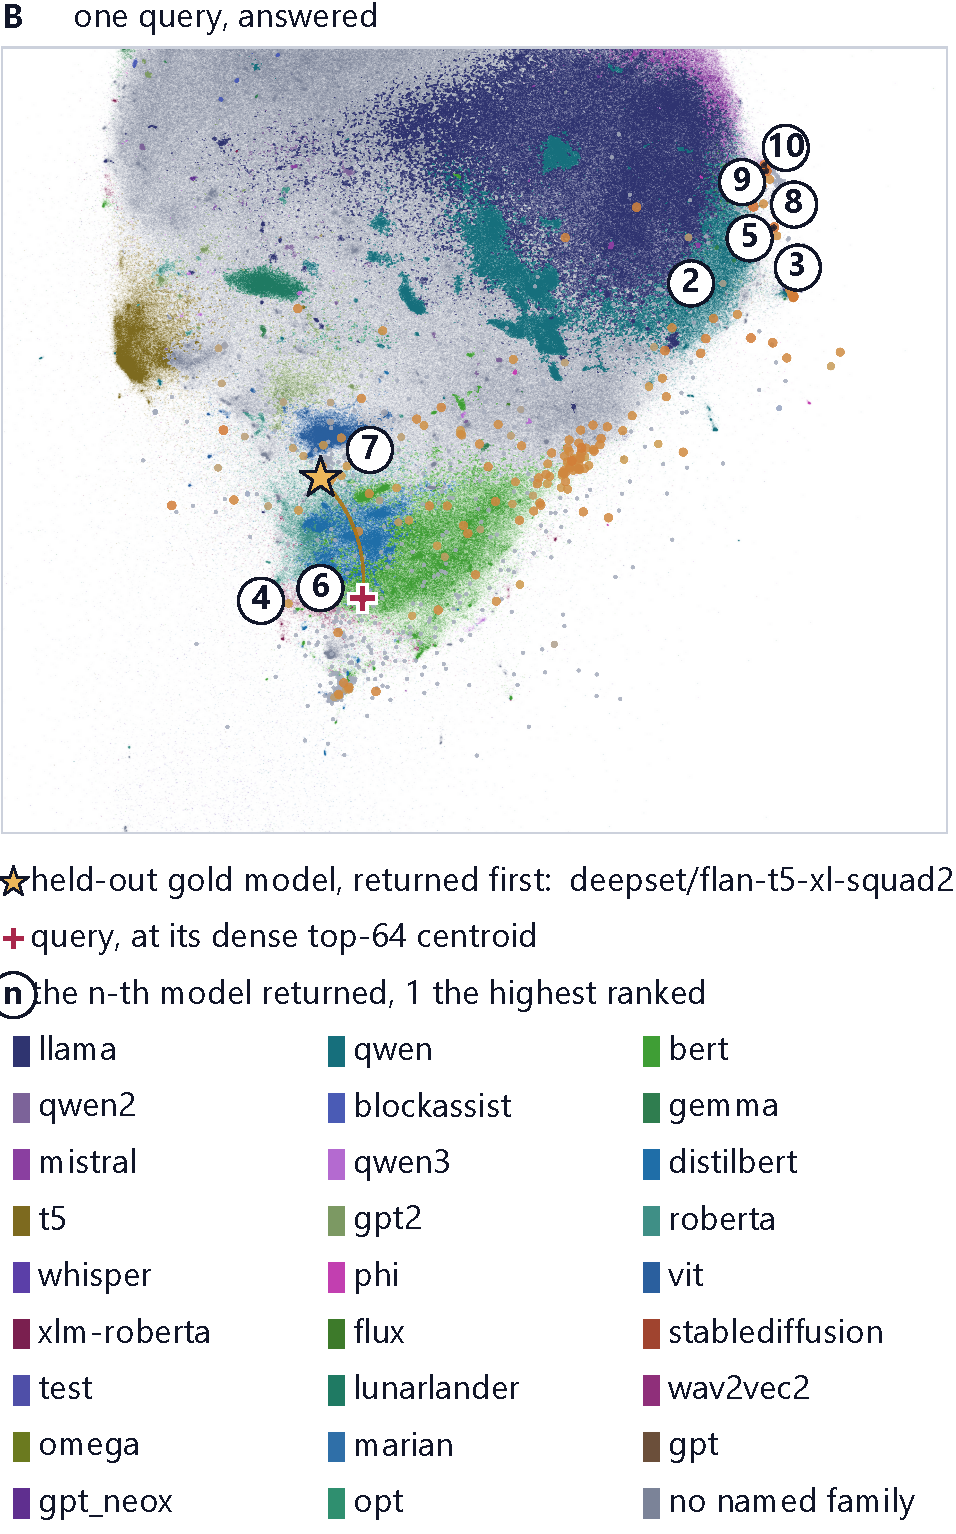
\includegraphics[width=\columnwidth]{figures/lake_b.pdf}
  \caption{%
    \textbf{One query, answered.} The $1{,}000$ candidates HNSW returned for
    the held-out query \texttt{squad}\,/\,\emph{question-answering}, coloured
    and sized by the task prior the second stage reads over them. Numbered
    discs are the ten models finally returned, in returned order; a disc
    nudged off its model keeps a hairline back to it. The gold star is the
    held-out best model, \texttt{deepset/flan-t5-xl-squad2}. Cosine alone
    ranks it $445$th of the pool; after the task-prior rerank it is returned
    first.%
  }
  \label{fig:lake-b}
\end{figure}


% -------------------------------------------------------------- both, in one --
% Two-column float, if you would rather have a single figure.
\begin{figure*}[t]
  \centering
  \includegraphics[width=\textwidth]{figures/lake_ab.pdf}
  \caption{%
    \textbf{Retrieval in a three-million-model lake.}
    \textbf{(A)} All $3{,}016{,}439$ model representations laid out once, as
    log density over a UMAP projection of the shared $128$-dimensional space;
    $64{,}086$ rows fall outside the frame, and neighbourhoods are meaningful
    while absolute distances are not. Labels mark the densest region of $17$
    of the $41{,}056$ model families. The crimson marker is the held-out query
    \texttt{squad}\,/\,\emph{question-answering}, and the amber outline
    encloses the region its $1{,}000$ retrieved candidates occupy.
    \textbf{(B)} The same query, enlarged. Every dot is one of those $1{,}000$
    candidates HNSW returned, coloured and sized by the task prior applied in
    the second stage; numbered discs are the ten models finally returned, in
    returned order. The gold star is the held-out best model,
    \texttt{deepset/flan-t5-xl-squad2}: cosine alone ranks it $445$th of
    the pool, and the rerank returns it
    \emph{first}. Both panels are drawn from the same A0 seed-0 export and
    graph as all reported numbers, and the cast is the measured seed-0
    retrieval rather than a recomputation.%
  }
  \label{fig:lake}
\end{figure*}


% -------------------------------------------------------------- short forms --
% If the float is tight, any of these works as a one-sentence caption.
%
% A:  The model lake: all 3,016,439 models in one shared retrieval space, with
%     17 families named and the region retrieved for a held-out query outlined
%     in amber.
%
% B:  Of the 1,000 candidates HNSW returns for a held-out query, the task-prior
%     rerank returns the held-out best model first, up from 445th on cosine
%     alone.
%
% AB: Retrieval in a three-million-model lake. (A) All 3,016,439 models in one
%     shared space, with the region retrieved for a held-out query outlined in
%     amber. (B) That query enlarged: of its 1,000 candidates the held-out best
%     model, 445th by cosine alone, is returned first.
